\documentclass[11pt,a4paper]{article}
\usepackage[utf8]{inputenc}
\usepackage{amsmath}
\usepackage{amsfonts}
\usepackage{amssymb}
\usepackage{graphicx}
\newcommand{\qed}{\hfill $\blacksquare$}
\author{Jake Bruner}
\title{Proof without words - Exploration}
\begin{document}
\maketitle
\tableofcontents
\pagebreak

\section{Introduction and Aim}

Calculating percent uncertainty slope

\begin{align*}
\textit{best fit slope} &= 3.332 \\
\textit{min slope} &= 3.155 \\
\textit{max slope} &= 3.538 
\end{align*}


$|m_{best} - m_{min/max}|$\\


Deviation from the Best Fit slope:

\begin{align*}
min \Delta = 0.177 \\
max \Delta = 0.206
\end{align*}

\begin{align*}
&=\frac{|m_{best} - m_{min/max}|}{m_{best}}\\
&=\frac{0.206}{3.332}\\
&= 6.18 \%
\end{align*}

\begin{align*}
\rho &= \frac{m}{A}\\
\rho &= \frac{m}{\pi r^2 h}\\
m &= \underbrace{(\rho \pi r^2)}_{slope} h \\ \\
\Rightarrow \rho &= \frac{slope}{\pi r^2}
\end{align*}

\begin{align*}
\rho &= \frac{3.332\ g\  cm^{-1}}{\pi(\frac{1}{2}1.25cm)^2}\\
\rho &= 2.715\ g\ cm^{-3}
\end{align*}

\iffalse
\pagebreak
\section{Understanding Proof Through Pythagoras}
\subsection{The First Proof \textit{circa} 200 BCE}
\begin{figure}[h]
\begin{center}
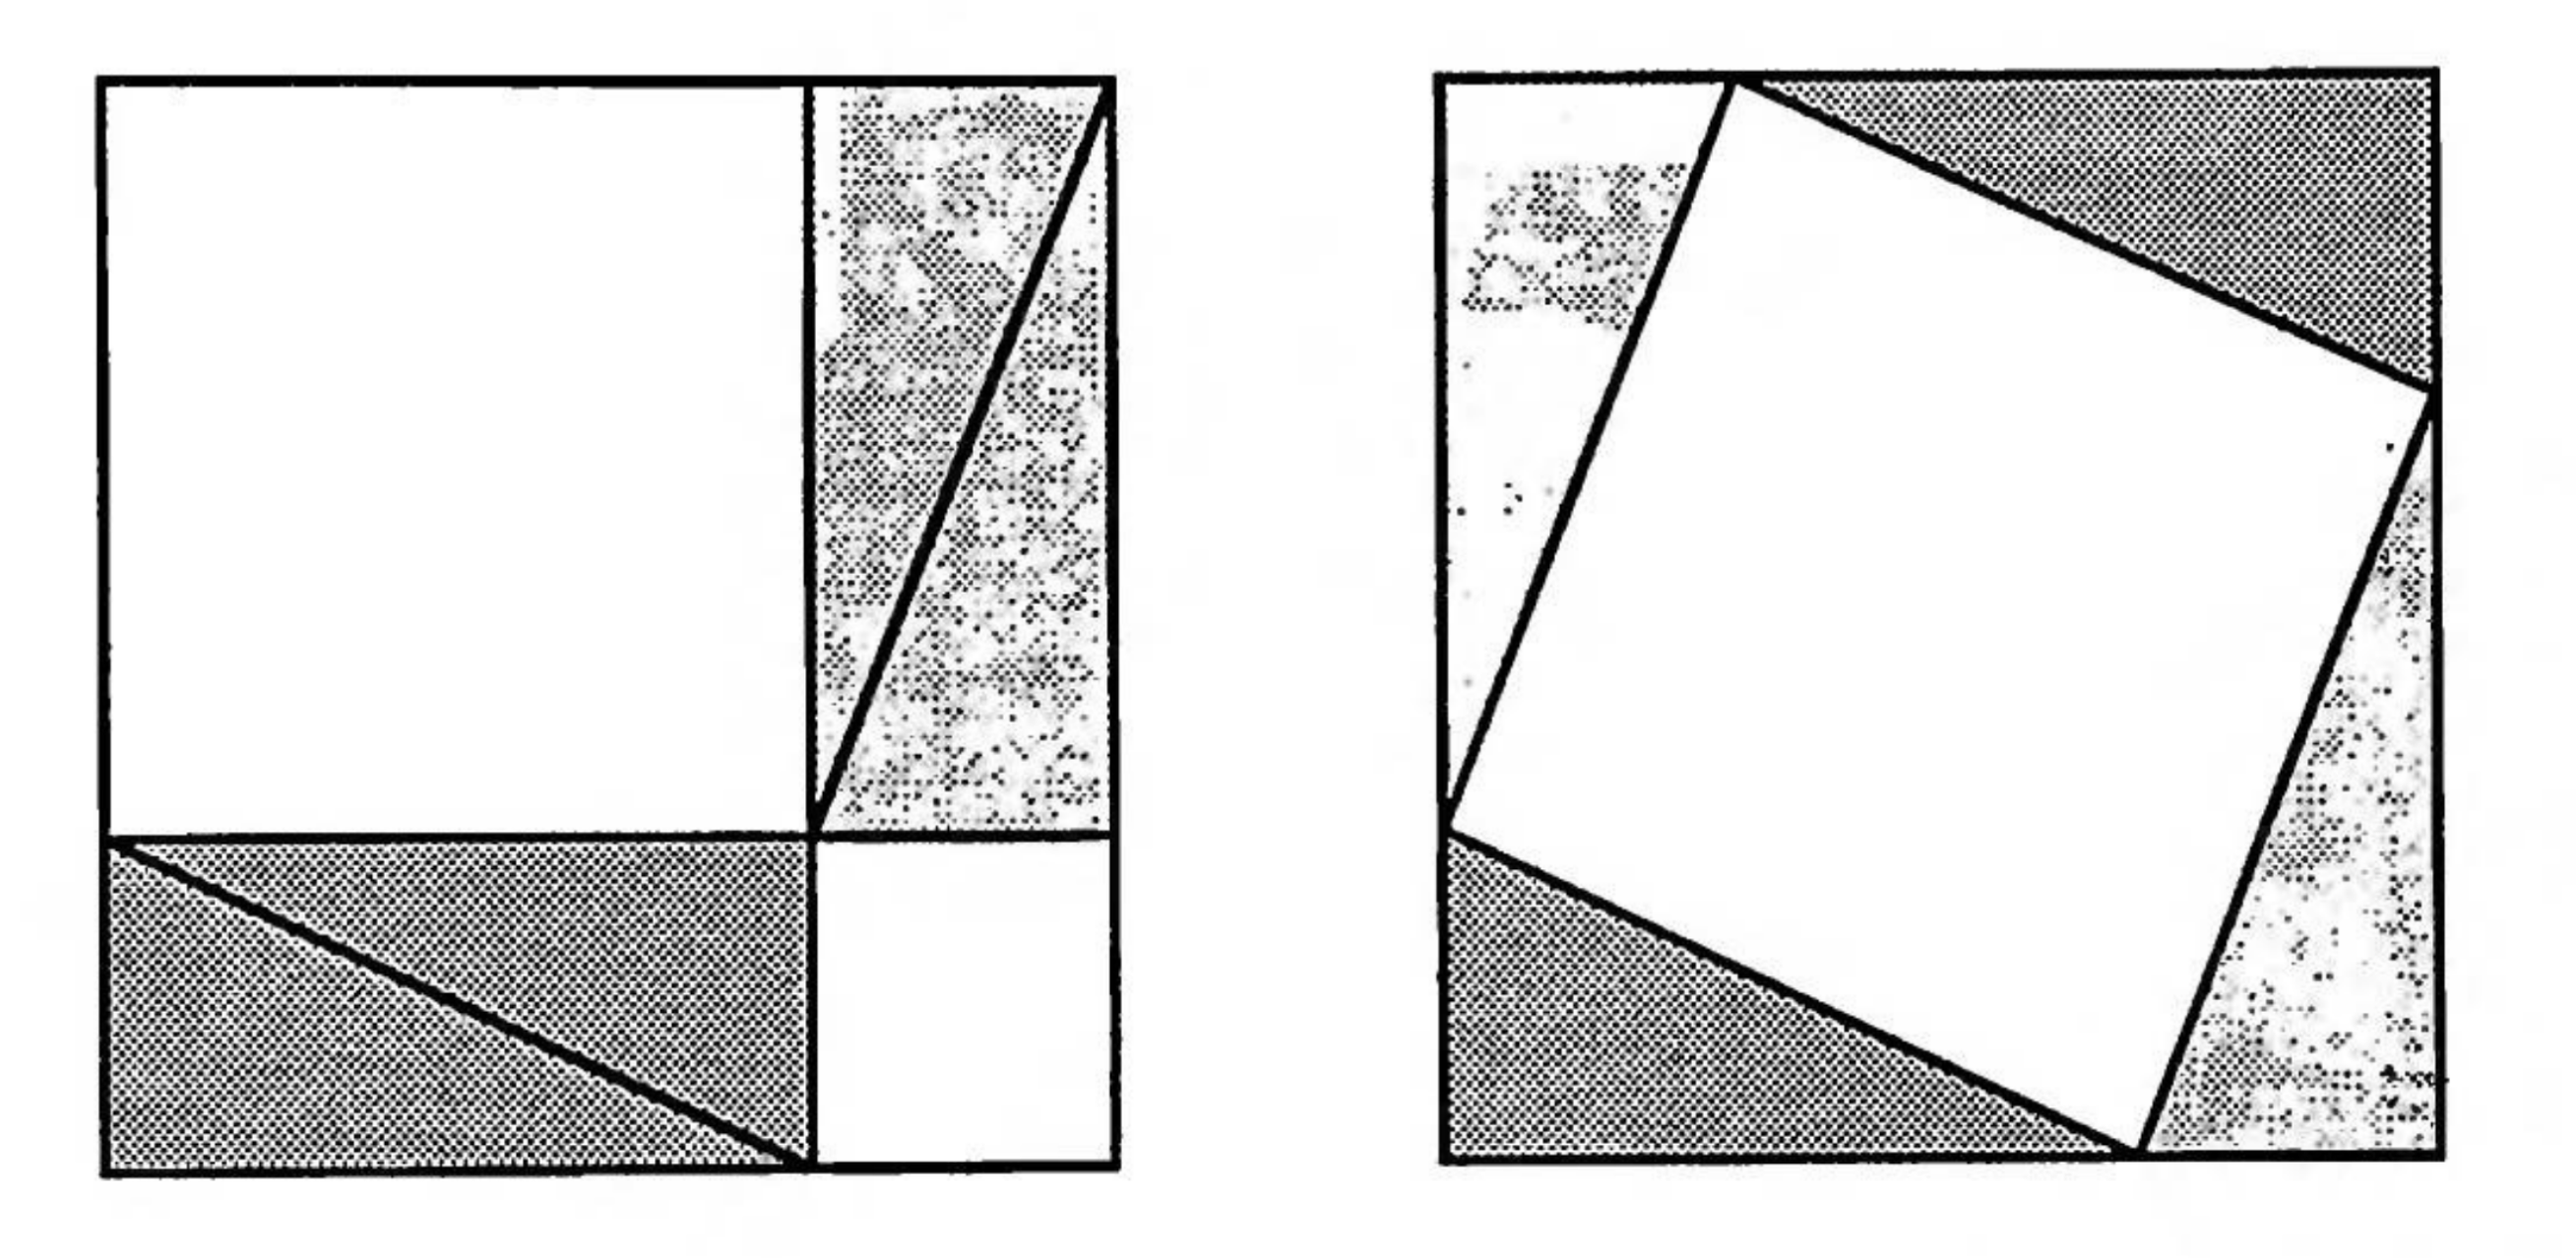
\includegraphics[scale=.20]{proof of pt} 
\caption{Proof of Pythagorean Theorem circa \textit{200 BC}}
\end{center}
\end{figure}
\fi


\end{document}
